% Шаблон для отчетов пол лабораторным работам в СПбГЭТУ "ЛЭТИ"
% Ефремов М.А. 2017г
%=== Тип документа - статья, кегль 14пт.
\documentclass[14pt]{article}
%=== Настройка кодировок, шрифта и языка
\usepackage[utf8]{inputenc}
\usepackage{extsizes}
\usepackage[main=russian, english]{babel}
\usepackage[T2A, T1]{fontenc}
%=== Разметка документа
\usepackage{geometry} 
\geometry{
	a4paper, 
	top = 2cm,
	bottom = 2cm,
	left = 3cm,
	right = 1cm
}
%=== Форматирование текста
\usepackage {setspace}			% Интерлиньяж
\onehalfspacing					% 1.5 строки
\usepackage {indentfirst} 		% Красная строка с первого предложения
\setlength						% Отступ красной строки - 1.25см
	{\parindent}
	{1.25cm}	
\usepackage {titlesec}			% Форматирование заголовков
% разделов
\titleformat
	{\section}
	[hang]
	{\normalsize\bfseries}
	{}{0pt}{}
\titlespacing
	{\section}
	{\parindent}
	{4ex}
	{0pt}
% подразделов (нумеруются)
\titleformat
	{\subsection}
	[hang]
	{\normalsize\bfseries\itshape}
	{\arabic{subsection}. }{0pt}{}
\titlespacing
	{\subsection}
	{\parindent}
	{4ex}
	{0pt}
%=== Минимизируем количество переносов
\usepackage {ragged2e}
\usepackage {microtype}
\tolerance = 500
\hyphenpenalty = 20000
\emergencystretch = 1cm
%=== Таблицы
\usepackage {tabularx}	% основной тип таблиц, выравнивание по ширине
\usepackage {longtable}	% для таблиц, не вмещающихся на одну страницу
\usepackage {multirow}	% для разбиения ячеек на несколько строк
\usepackage {multicol}	% на несколько колонок
%=== ^ до этого места - минимальная преамбула документа.
%=== Далее идут опциональные, но часто использущиеся пакеты,
%=== а так же написанные мной команды, чем-то упрощающие написание отчетов

%=== Работа с формулами
% Набор пакетов, сильно расширяющих возможности по набору формул
\usepackage{amsmath}
% добавляет специфические для русских  статей мат. символы вроде \leqslant
\usepackage{amssymb}
% добавляет окружения для теорем и лемм	
\usepackage{amsthm}				
\usepackage{mathtools}
% номера только для тех формул, на которые есть ссылки в тексте
\mathtoolsset{showonlyrefs=true}

%=== Работа с изображениями
\usepackage{graphicx}
\usepackage{caption}
\usepackage{subcaption}

%=== Работа с гиперссылками
\usepackage{hyperref}
\hypersetup{
	colorlinks=true,
	urlcolor=blue,
	filecolor=green,
	linkcolor=red
}

%=== Вставка кода
\usepackage{listings}
\usepackage{xcolor}
\lstset { %
	basicstyle = \footnotesize,% basic font setting
	captionpos = b,
	numbers    = left,
	frame      = single
}

% Компиляция под Windows 10 при помощи XeLaTeX для использования шрифта Times New Roman
\usepackage{fontspec}
\setmainfont{Times New Roman}

\begin{document}
	\pagenumbering{gobble}
\clearpage
\begin{center}	
	МИНОБРНАУКИ РОССИИ\\
	САНКТ-ПЕТЕРБУРГСКИЙ ГОСУДАРСТВЕННЫЙ\\
	ЭЛЕКТРОТЕХНИЧЕСКИЙ УНИВЕРСИТЕТ\\
	«ЛЭТИ» ИМ. В.И. УЛЬЯНОВА (ЛЕНИНА)\\
	Кафедра МО ЭВМ

	\vspace{54mm}

	ОТЧЕТ\\
	по лабораторной работе №1 \\
	по дисциплине «Алгоритмы компьютерного зрения» \\
	Тема: калибровка камеры \\

	\vspace{65mm}

	\def\arraystretch{1.5}
	\begin{tabularx}{\textwidth}{ >{\hsize=7cm}X >{\hsize=4.1cm}X  >{\centering\arraybackslash}X }
		Студент гр. 2304 & & Ефремов М.А. \\ \cline{2-2}
		Преподаватель & & Черниченко Д.А. \\ \cline{2-2}
	\end{tabularx}
	\def\arraystretch{1}

	\vfill
	Санкт-Петербург\\
	2017
\end{center}
\newpage
\pagenumbering{arabic}
\setcounter{page}{1}
	
	\section{Цель работы.}
		При помощи библиотеки OpenCV, используя предложенные изображения в качестве входных данных, получить карту глубины.
	
	\section{Основные теоретические положения.}
		Карта глубины — это изображение, на котором для каждого пикселя, вместо цвета, храниться его расстояние до камеры. Карта глубины может быть построена по стереопаре изображений.

Идея, лежащая в основе построения карты глубины по стереопаре следующая: для каждой точки на одном изображении выполняется поиск парной ей точки на другом изображении. По паре соответствующих точек можно выполнить триангуляцию и определить координаты их прообраза в трехмерном пространстве. Зная трехмерные координаты прообраза, глубина вычисляется, как расстояние до плоскости камеры.

Парную точку нужно искать на эпиполярной линии. Для упрощения поиска, изображения выравнивают так, что бы все эпиполярные линии были параллельны сторонам изображения (обычно горизонтальны). Изображения выравнивают так, что бы для точки с координатами $(x_0, y_0)$ соответствующая ей эпиполярная линия задавалась уравнением $x = x_0$, тогда для каждой точки соответствующую ей парную точку нужно искать в той-же строчке на изображении со второй камеры. Такой процесс выравнивания изображений называют ректификацией. Обычно ректификацию совершают путем ремаппинга изображения и ее совмещают с избавлением от дисторсий.

После того как изображения ректифицированы, выполняют поиск соответствующих пар точек. Самый простой способ проиллюстрирован на рисунке \ref{img:approach} и состоит в следующем: для каждого пикселя левой картинки с координатами $(x_0, y_0)$ выполняется поиск пикселя на правой картинке. При этом предполагается, что пиксель на правой картинке должен иметь координаты $(x_0 - d, y_0)$, где $d$ — величина называемая несоответствием или смещением (disparity). Поиск соответствующего пикселя выполняется путем вычисления максимума функции отклика, в качестве которой может выступать, например, корреляция окрестностей пикселей.

\begin{figure}[!h]
	\center {
		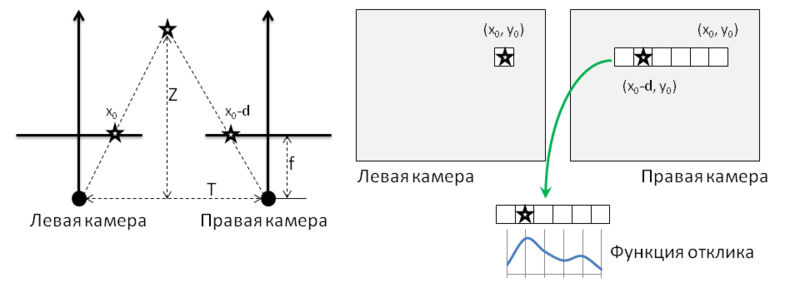
\includegraphics[width=\linewidth]{img/approach}
	}
	\caption{Метод поиска соответствующих пар проекций точек на стереопару.}
	\label{img:approach}
\end{figure}
	
	\section{Программа.}
		Далее на листинге \ref{lst:code} приведена программа, написанная для построения карты глубины. 

\begin{lstlisting} [language = C++, caption = {Получение карты глубины} ,label={lst:code}]
#include "opencv2/imgcodecs.hpp"
#include "opencv2/imgproc.hpp"
#include "opencv2/calib3d/calib3d.hpp"

using namespace cv;
using namespace std;

int main()
{
	String img_names[2];
	img_names[0] = "images/right1.jpg"; 
	img_names[1] = "images/right2.jpg";
	
	vector<Mat> imgs;
	for (int i = 0; i < 2; ++i) {
		Mat img = imread(img_names[i], 0);
		imgs.push_back(img);
	}
	
	Mat disp, disp8;
	Ptr<StereoBM> bm = StereoBM::create(16, 5);
	bm->compute(imgs.at(0), imgs.at(1), disp);
	imwrite("depth_map_result.jpg", disp);
	
	return 0;
}
\end{lstlisting}
		
	\section{Экспериментальные результаты.}
		За основу был взят пример на OpenCV, вычисляющие и выдающий в формате xml требующиеся параметры камеры. Программа принимает на вход xml файл с настройками. Для упрощения работы файлу было дано имя default.xml, которое не надо указывать для запуска программы. В нем были указаны входные данные: размер шахматной доски 14 в ширину и 10 в высоту, количество снимков - 15, путь до xml файла, описывающий местонахождение снимков.

Исходный код идентичен примеру 3calibration.cpp, собранный проект доступен в репозитории: \url{https://github.com/JAkutenshi/ma_2sem_cva/tree/master/Camera_Calibration}. В этом репозитории, в файле \textit{out\_camera\_data.xml } хранится результат программы.

Полученные результаты представлены в выражениях \eqref{eq:k_result} и \eqref{eq:c_distorce_result}.

\begin{equation}\label{eq:k_result}
K_{ideal} = 
\begin{pmatrix}
1189.273 & 0 		& 384 \\
0		 & 1189.273 & 290 \\ 
0		 & 0		& 1 
\end{pmatrix}
\end{equation}
\begin{equation}\label{eq:c_distorce_result}
C_{distorceIdeal} = 
\left[
\begin{array}{ccccc}
-0.346 & 1.698 & 0 & 0 & -5.537
\end{array}
\right]
\end{equation}

	\section{Выводы.}
		В результате выполнения программы была получена карта глубины, но, скорее-всего из-за большого расстояния до объектов, ее точность оставляет желать лучшего. т.к. явно более далекие объекты не всегда отличимы от близких. Ближайшие объекты шкаф и тумбочка и они находятся достаточно далеко от камеры.

\end{document}